% Created by tikzDevice version 0.8.1 on 2015-10-21 20:58:30
% !TEX encoding = UTF-8 Unicode
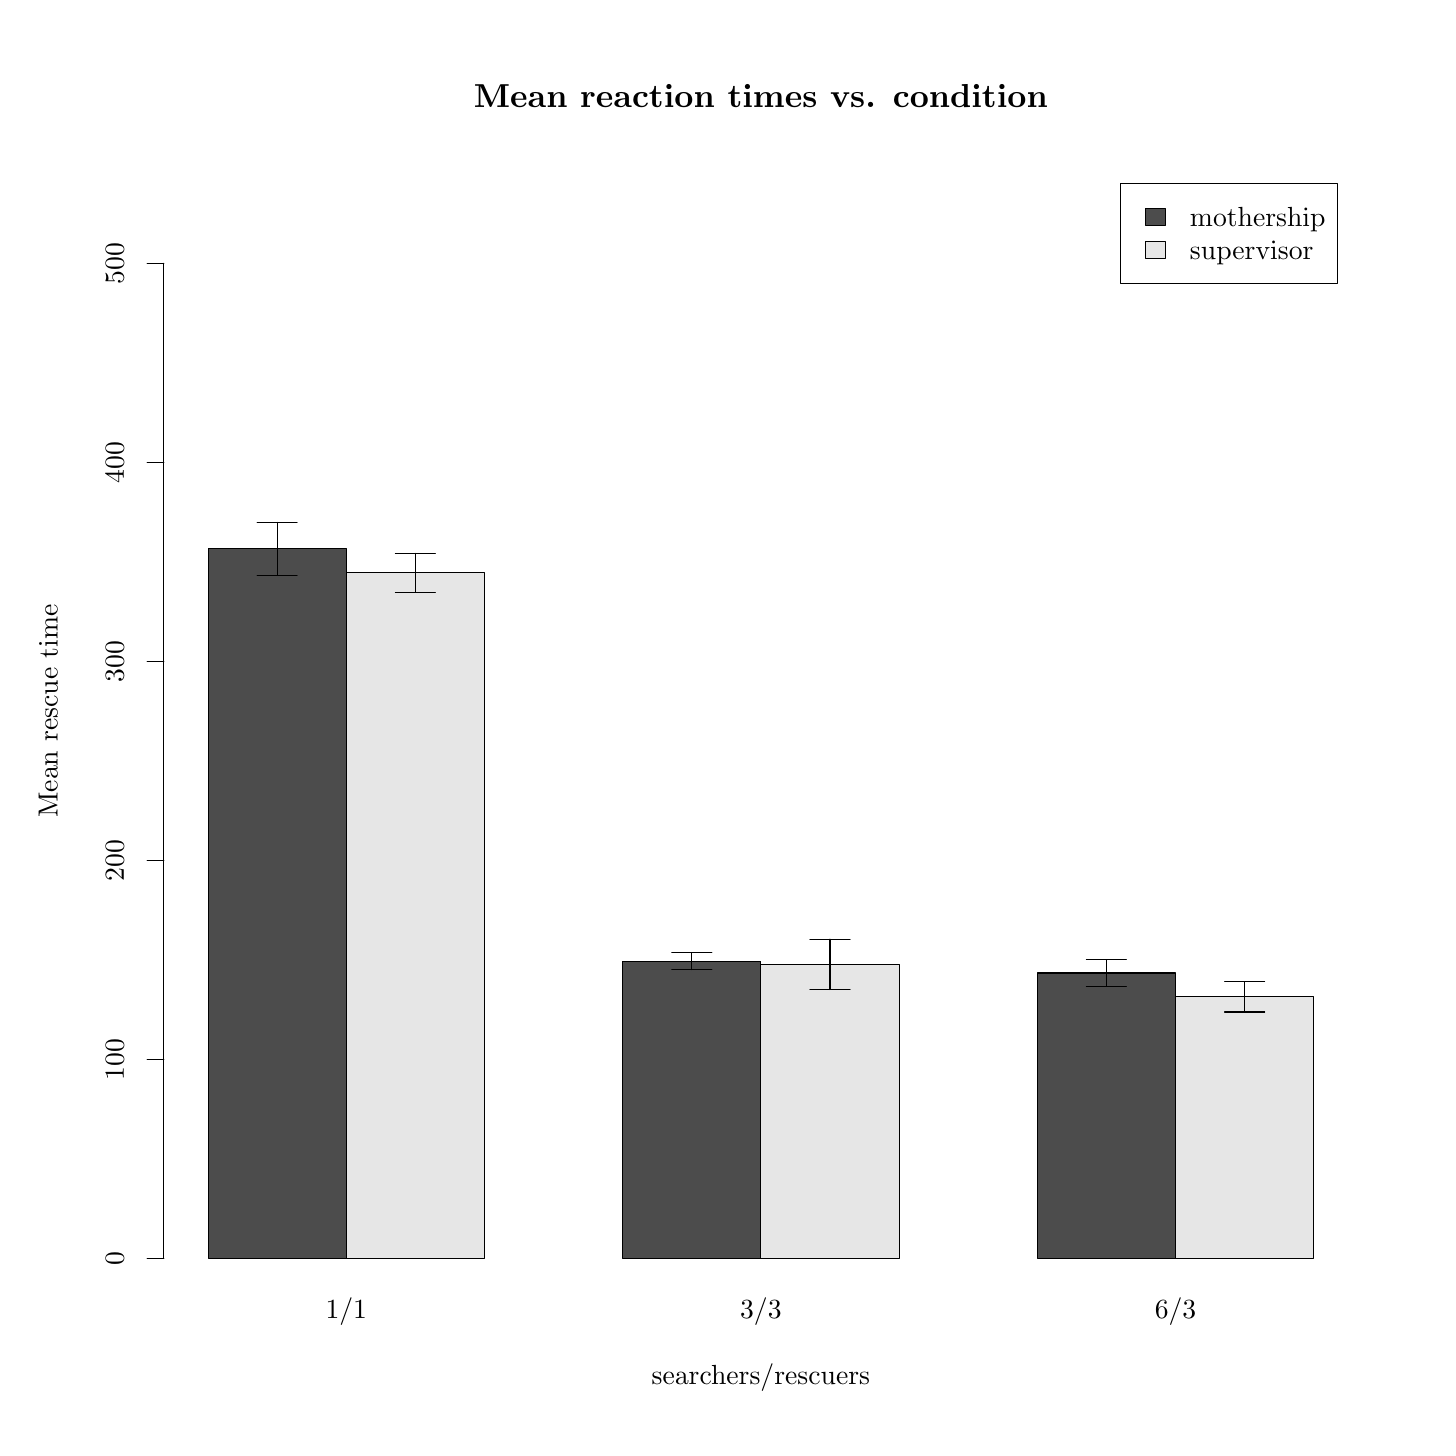
\begin{tikzpicture}[x=1pt,y=1pt]
\definecolor{fillColor}{RGB}{255,255,255}
\path[use as bounding box,fill=fillColor,fill opacity=0.00] (0,0) rectangle (505.89,505.89);
\begin{scope}
\path[clip] (  0.00,  0.00) rectangle (505.89,505.89);
\definecolor{drawColor}{RGB}{0,0,0}
\definecolor{fillColor}{gray}{0.30}

\path[draw=drawColor,line width= 0.4pt,line join=round,line cap=round,fill=fillColor] ( 65.18, 61.20) rectangle (115.12,317.54);
\definecolor{fillColor}{RGB}{230,230,230}

\path[draw=drawColor,line width= 0.4pt,line join=round,line cap=round,fill=fillColor] (115.12, 61.20) rectangle (165.06,308.86);
\definecolor{fillColor}{gray}{0.30}

\path[draw=drawColor,line width= 0.4pt,line join=round,line cap=round,fill=fillColor] (215.00, 61.20) rectangle (264.94,168.56);
\definecolor{fillColor}{RGB}{230,230,230}

\path[draw=drawColor,line width= 0.4pt,line join=round,line cap=round,fill=fillColor] (264.94, 61.20) rectangle (314.89,167.42);
\definecolor{fillColor}{gray}{0.30}

\path[draw=drawColor,line width= 0.4pt,line join=round,line cap=round,fill=fillColor] (364.83, 61.20) rectangle (414.77,164.31);
\definecolor{fillColor}{RGB}{230,230,230}

\path[draw=drawColor,line width= 0.4pt,line join=round,line cap=round,fill=fillColor] (414.77, 61.20) rectangle (464.71,155.68);
\end{scope}
\begin{scope}
\path[clip] (  0.00,  0.00) rectangle (505.89,505.89);
\definecolor{drawColor}{RGB}{0,0,0}

\node[text=drawColor,anchor=base,inner sep=0pt, outer sep=0pt, scale=  1.00] at (115.12, 39.60) {1/1};

\node[text=drawColor,anchor=base,inner sep=0pt, outer sep=0pt, scale=  1.00] at (264.94, 39.60) {3/3};

\node[text=drawColor,anchor=base,inner sep=0pt, outer sep=0pt, scale=  1.00] at (414.77, 39.60) {6/3};
\end{scope}
\begin{scope}
\path[clip] (  0.00,  0.00) rectangle (505.89,505.89);
\definecolor{drawColor}{RGB}{0,0,0}

\path[draw=drawColor,line width= 0.4pt,line join=round,line cap=round] (394.80,449.46) rectangle (473.46,413.46);
\definecolor{fillColor}{gray}{0.30}

\path[draw=drawColor,line width= 0.4pt,line join=round,line cap=round,fill=fillColor] (403.80,440.46) rectangle (411.00,434.46);
\definecolor{fillColor}{RGB}{230,230,230}

\path[draw=drawColor,line width= 0.4pt,line join=round,line cap=round,fill=fillColor] (403.80,428.46) rectangle (411.00,422.46);

\node[text=drawColor,anchor=base west,inner sep=0pt, outer sep=0pt, scale=  1.00] at (420.00,434.02) {mothership};

\node[text=drawColor,anchor=base west,inner sep=0pt, outer sep=0pt, scale=  1.00] at (420.00,422.02) {supervisor};

\node[text=drawColor,anchor=base,inner sep=0pt, outer sep=0pt, scale=  1.20] at (264.94,477.15) {\bfseries Mean reaction times vs. condition};

\node[text=drawColor,anchor=base,inner sep=0pt, outer sep=0pt, scale=  1.00] at (264.94, 15.60) {searchers/rescuers};

\node[text=drawColor,rotate= 90.00,anchor=base,inner sep=0pt, outer sep=0pt, scale=  1.00] at ( 10.80,258.94) {Mean rescue time};
\end{scope}
\begin{scope}
\path[clip] (  0.00,  0.00) rectangle (505.89,505.89);
\definecolor{drawColor}{RGB}{0,0,0}

\path[draw=drawColor,line width= 0.4pt,line join=round,line cap=round] ( 49.20, 61.20) -- ( 49.20,420.74);

\path[draw=drawColor,line width= 0.4pt,line join=round,line cap=round] ( 49.20, 61.20) -- ( 43.20, 61.20);

\path[draw=drawColor,line width= 0.4pt,line join=round,line cap=round] ( 49.20,133.11) -- ( 43.20,133.11);

\path[draw=drawColor,line width= 0.4pt,line join=round,line cap=round] ( 49.20,205.01) -- ( 43.20,205.01);

\path[draw=drawColor,line width= 0.4pt,line join=round,line cap=round] ( 49.20,276.92) -- ( 43.20,276.92);

\path[draw=drawColor,line width= 0.4pt,line join=round,line cap=round] ( 49.20,348.83) -- ( 43.20,348.83);

\path[draw=drawColor,line width= 0.4pt,line join=round,line cap=round] ( 49.20,420.74) -- ( 43.20,420.74);

\node[text=drawColor,rotate= 90.00,anchor=base,inner sep=0pt, outer sep=0pt, scale=  1.00] at ( 34.80, 61.20) {0};

\node[text=drawColor,rotate= 90.00,anchor=base,inner sep=0pt, outer sep=0pt, scale=  1.00] at ( 34.80,133.11) {100};

\node[text=drawColor,rotate= 90.00,anchor=base,inner sep=0pt, outer sep=0pt, scale=  1.00] at ( 34.80,205.01) {200};

\node[text=drawColor,rotate= 90.00,anchor=base,inner sep=0pt, outer sep=0pt, scale=  1.00] at ( 34.80,276.92) {300};

\node[text=drawColor,rotate= 90.00,anchor=base,inner sep=0pt, outer sep=0pt, scale=  1.00] at ( 34.80,348.83) {400};

\node[text=drawColor,rotate= 90.00,anchor=base,inner sep=0pt, outer sep=0pt, scale=  1.00] at ( 34.80,420.74) {500};
\end{scope}
\begin{scope}
\path[clip] ( 49.20, 61.20) rectangle (480.69,456.69);
\definecolor{drawColor}{RGB}{0,0,0}

\path[draw=drawColor,line width= 0.4pt,line join=round,line cap=round] ( 90.15,307.99) -- ( 90.15,327.08);

\path[draw=drawColor,line width= 0.4pt,line join=round,line cap=round] ( 82.92,307.99) --
	( 90.15,307.99) --
	( 97.38,307.99);

\path[draw=drawColor,line width= 0.4pt,line join=round,line cap=round] ( 97.38,327.08) --
	( 90.15,327.08) --
	( 82.92,327.08);

\path[draw=drawColor,line width= 0.4pt,line join=round,line cap=round] (140.09,301.84) -- (140.09,315.89);

\path[draw=drawColor,line width= 0.4pt,line join=round,line cap=round] (132.87,301.84) --
	(140.09,301.84) --
	(147.32,301.84);

\path[draw=drawColor,line width= 0.4pt,line join=round,line cap=round] (147.32,315.89) --
	(140.09,315.89) --
	(132.87,315.89);

\path[draw=drawColor,line width= 0.4pt,line join=round,line cap=round] (239.97,165.49) -- (239.97,171.63);

\path[draw=drawColor,line width= 0.4pt,line join=round,line cap=round] (232.75,165.49) --
	(239.97,165.49) --
	(247.20,165.49);

\path[draw=drawColor,line width= 0.4pt,line join=round,line cap=round] (247.20,171.63) --
	(239.97,171.63) --
	(232.75,171.63);

\path[draw=drawColor,line width= 0.4pt,line join=round,line cap=round] (289.92,158.35) -- (289.92,176.48);

\path[draw=drawColor,line width= 0.4pt,line join=round,line cap=round] (282.69,158.35) --
	(289.92,158.35) --
	(297.14,158.35);

\path[draw=drawColor,line width= 0.4pt,line join=round,line cap=round] (297.14,176.48) --
	(289.92,176.48) --
	(282.69,176.48);

\path[draw=drawColor,line width= 0.4pt,line join=round,line cap=round] (389.80,159.49) -- (389.80,169.14);

\path[draw=drawColor,line width= 0.4pt,line join=round,line cap=round] (382.57,159.49) --
	(389.80,159.49) --
	(397.02,159.49);

\path[draw=drawColor,line width= 0.4pt,line join=round,line cap=round] (397.02,169.14) --
	(389.80,169.14) --
	(382.57,169.14);

\path[draw=drawColor,line width= 0.4pt,line join=round,line cap=round] (439.74,150.21) -- (439.74,161.14);

\path[draw=drawColor,line width= 0.4pt,line join=round,line cap=round] (432.51,150.21) --
	(439.74,150.21) --
	(446.97,150.21);

\path[draw=drawColor,line width= 0.4pt,line join=round,line cap=round] (446.97,161.14) --
	(439.74,161.14) --
	(432.51,161.14);
\end{scope}
\end{tikzpicture}
